\end{multicols}
\begin{multicols}{2}[\section{Design}]
\label{sec:design}

In the following subsections our design decisions are briefly explained. A description of how these influenced our project and what we learned from them will be given in the \autoref{sec:outcomes}. The first section discusses our domain model. The second section deals with our data access layer. The third section is about our web application. The last section describes the scheduler algorithm.

\end{multicols}
\begin{multicols}{2}[\subsection{Domain model}]

Since universities are organized quite differently we tried to design the domain model as generic as possible. An important aspect of the application is reusability of course definitions. This requirement lead to the following design of course related information in our domain model.

\begin{description}
	\item [Course] is a well-defined set of \emph{CourseElements} and has only a name. For example the department of physics offers the course Thermodynamics.
	\item [CourseElement] is part of a \emph{Course} with a type and a duration. The course Thermodynamics consists of two \emph{CourseElements}, a two-hour lecture and a four-hour workshop.
	\item [CourseInstance] is a realization of a course for a specific program. The course Thermodynamics is held every second academic term. 
	\item [CourseElementInstance] is a realization of a \emph{CourseElement}, where several \emph{CourseElementInstances} constitute one \emph{CourseElement}. For instance the lecture is held on Monday from 10 to 12. The workshop on the other hand is divided into two events, that are held on Tuesday from 10 to 12 and Friday from 8 to 10.
\end{description}

Universities differ in their definitions of class types, features that a room may or may not have and features that a course may require. As such it appears to be infeasible to predefine these properties appropriately. Therefore our model allows universities to define the possible values of these properties. This generic modelling of properties is achieved by representing them as an attribute in a special entity. These entities are connected to the original entity indirectly through a relation that defines the connection.

\begin{figure}[H]
	\centering
		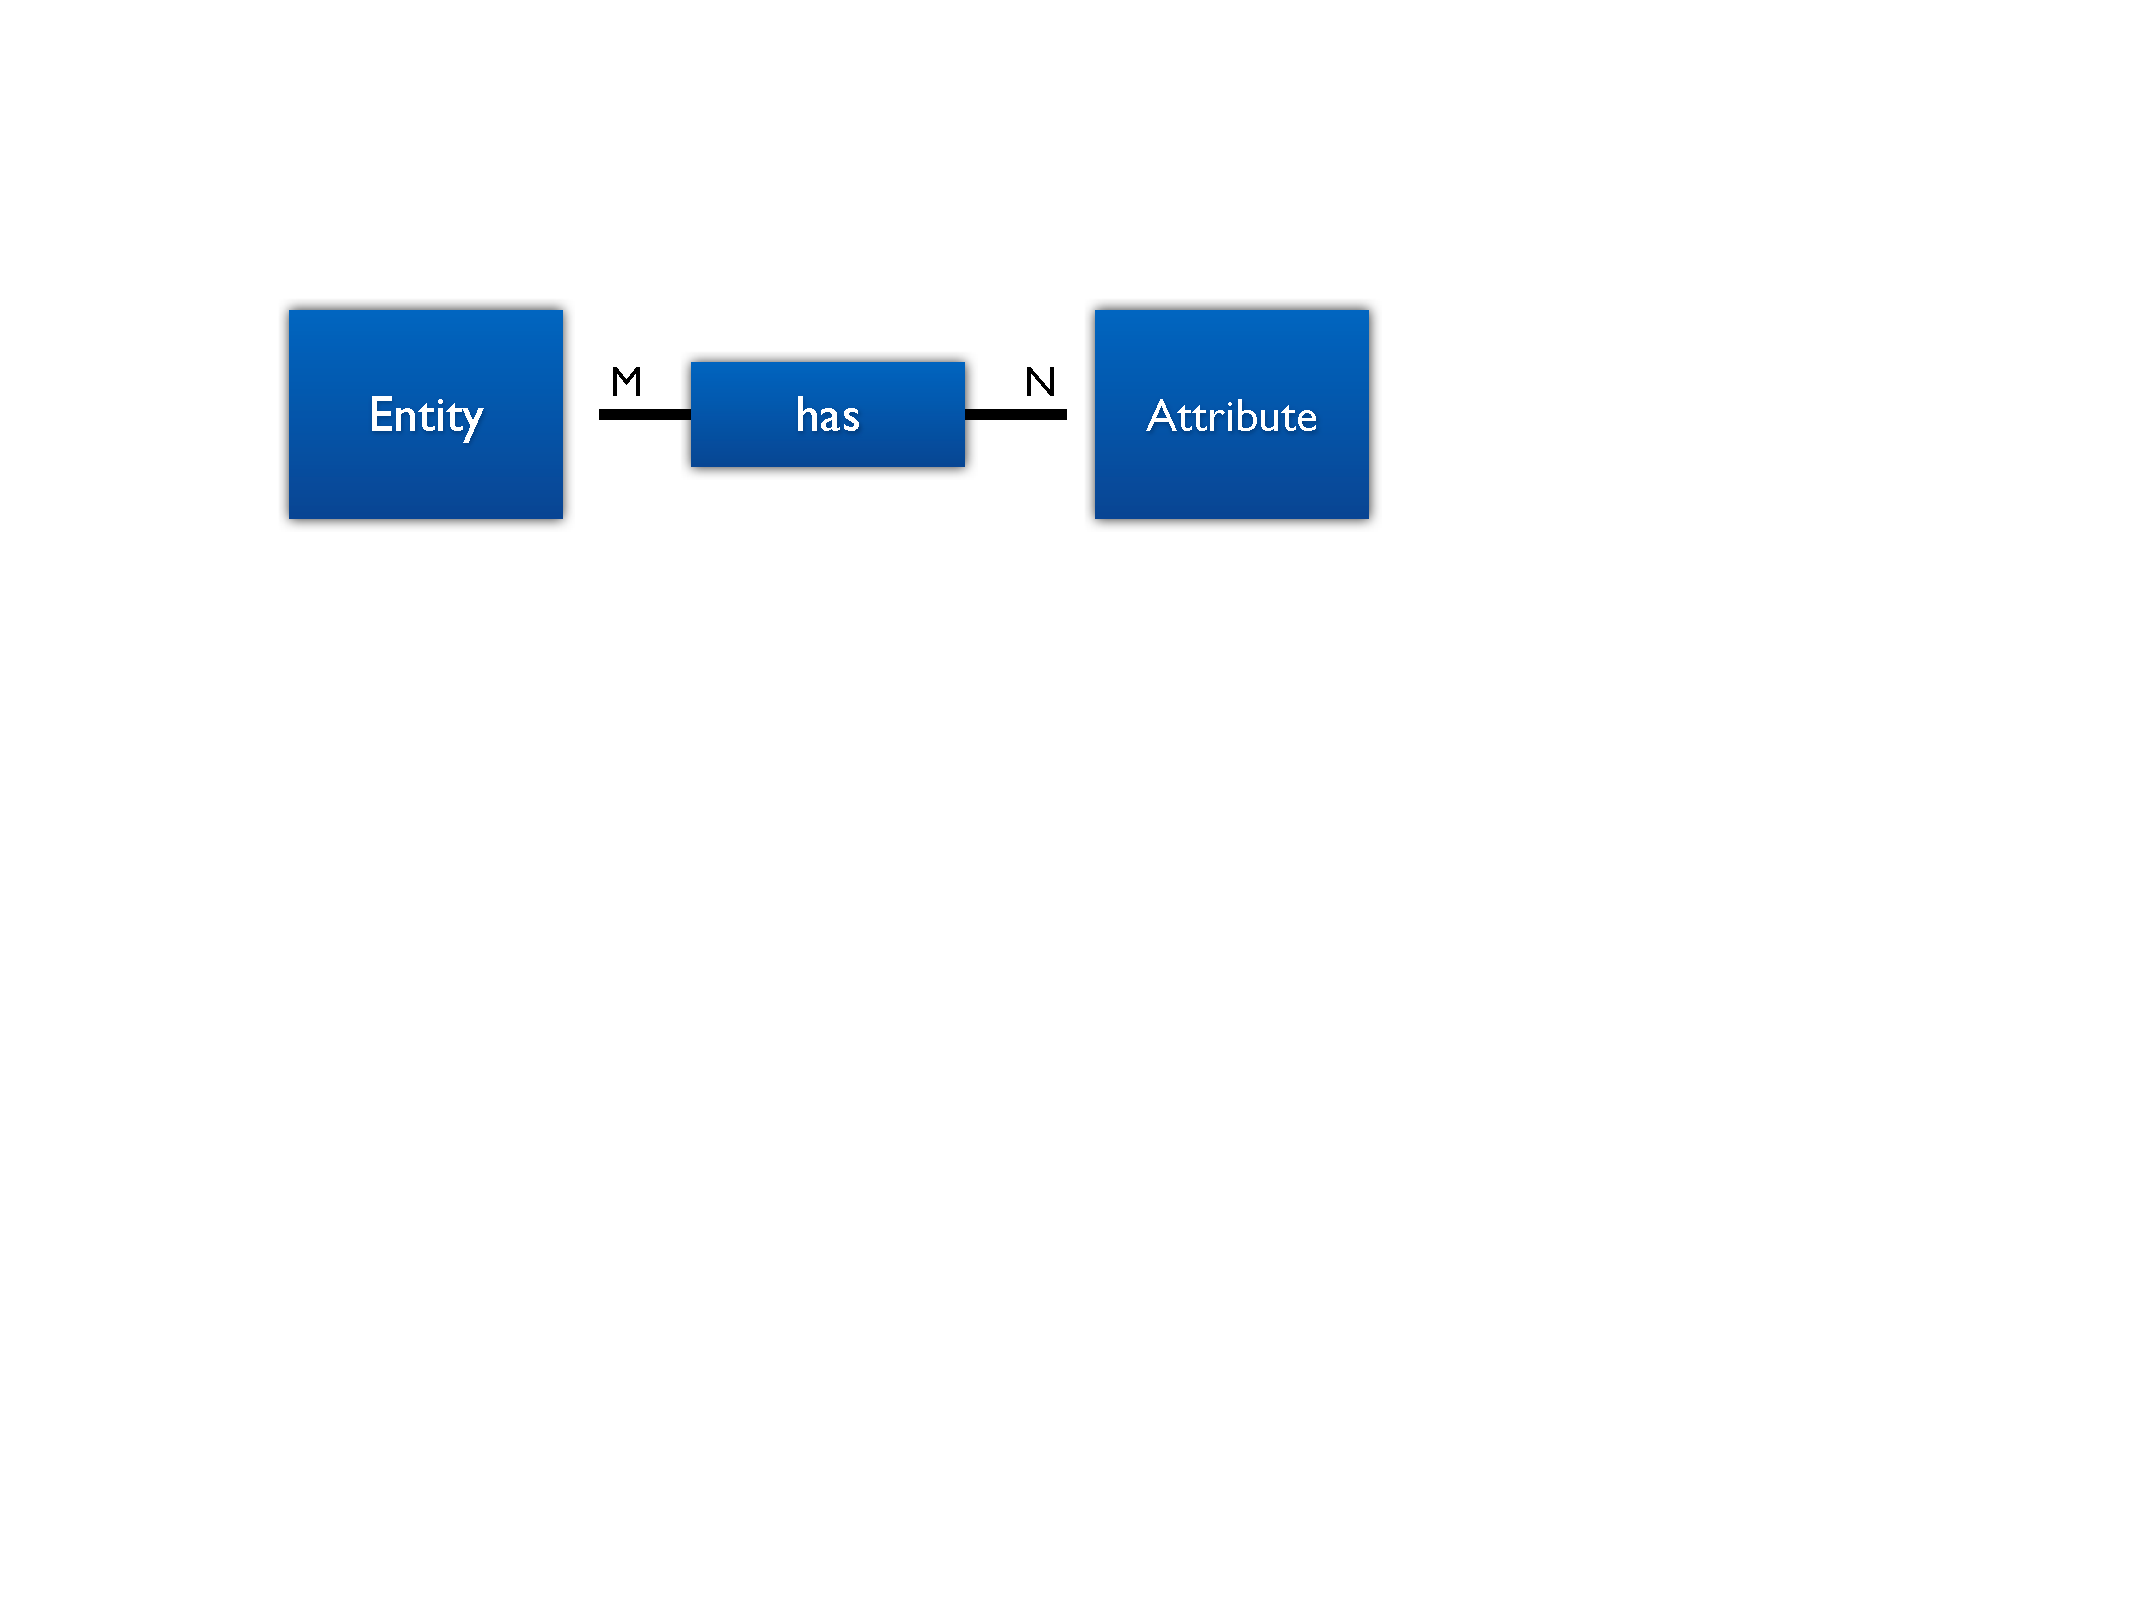
\includegraphics[width=\columnwidth]{images/orm_personroleprivilege.pdf}
	\caption{Many-to-many relation: generic model is achieved by representing them as an attribute in a
 special entity.}
	\label{fig:personroleprivilege}
\end{figure}

This also applies to user management where many different roles and sets of privileges are conceivable. Privileges themselves are predefined as they are a direct result of the possible actions. Furthermore universities might want to store additional information related to a course or person. The generic properties for Features of Rooms, CourseElements and CourseElementInstances are

\begin{itemize}
	\item CourseElement requires Feature
	\item CourseElementInstance requires Feature
	\item Room provides Feature
\end{itemize}

This means that for example a CourseElementInstance can have an arbitrary number of user defined Features. The connection is established through the relation CourseElementInstanceRequiresFeature. The connection can hold information about the minimum and maximum quantity, i.e. the number of seats a Room provides is represented in RoomProvidesFeature where the Feature has the name Seat.

\begin{itemize}
	\item Person has Attribute
	\item Course has CourseAttribute
\end{itemize}

Can be used to add user-defined attributes to a Person or a Course. For example the address of a Person can be stored as an Attribute.

\begin{itemize}
	\item Person has Role
	\item Role implies Privilege
	\item Person has Privilege
\end{itemize}

Are used by the user management to provide Privileges to groups  by RolImpliesPrivilege, or directly to Persons. For example the Role secretary may have user management Privileges. Furthermore the model enables a wide range of constraints.

\begin{itemize}
\item CourseElementInstance prefers Room

\item CourseElementInstance prefers Timeslot

\item Person prefers Timeslot

\item Room prefers Timeslot
\end{itemize}


\end{multicols}
\begin{multicols}{2}[\subsection{Data access layer}]

The object-relational model we defined deals with entities and relationships. Relationships connect two entities in a certain manner. Since they can have attributes too, we decided to model them as individual objects too, i.e. they are both represented as a table in the database as well as as a class in our object-oriented domain model. These classes implement the interfaces \emph{Entitiy} or \emph{Relationship} which in turn extend the interface Relation.

The objects should both represent the data as well as control the communication with the database, that means, they should be \emph{DAOs} (\emph{data access objects}) and \emph{DTOs} (\emph{data transfer objects}) at the same time. To accomplish this, we designed them as \emph{Active Records}. They feature methods to create, update and delete them. For retrieving data a special \emph{RelationManager} was defined. It is the central access point to the database and acts as a \emph{Factory} for the Active Records.

Since the code for the data access layer is auto generated its static structure follows a strict pattern. Each record has getters and setters to access the encapsulated data, the RelationManager has factory methods for each Entity and Relationship. Records that represent entities do also have special methods for retrieving datasets which are related via a special Relationship. One can now ask a Person-record which Privileges it has via PersonHasPrivilege-relationships, i.e. what the objects to the PersonHasPrivilege-relationship, in which that record is the subject, are. It is also possible to ask the other way around, i.e. what subjects are assigned to a given object via a certain relationship.

One key feature of the active records is, that if something (for example an attribute which represents a reference to another dataset) is requested which has not yet been retrieved from the database, it may transparently be fetched from the database. If, on the other hand, that record has already been fetched it may simply be loaded from a cache.

\begin{figure}[H]
	\centering
		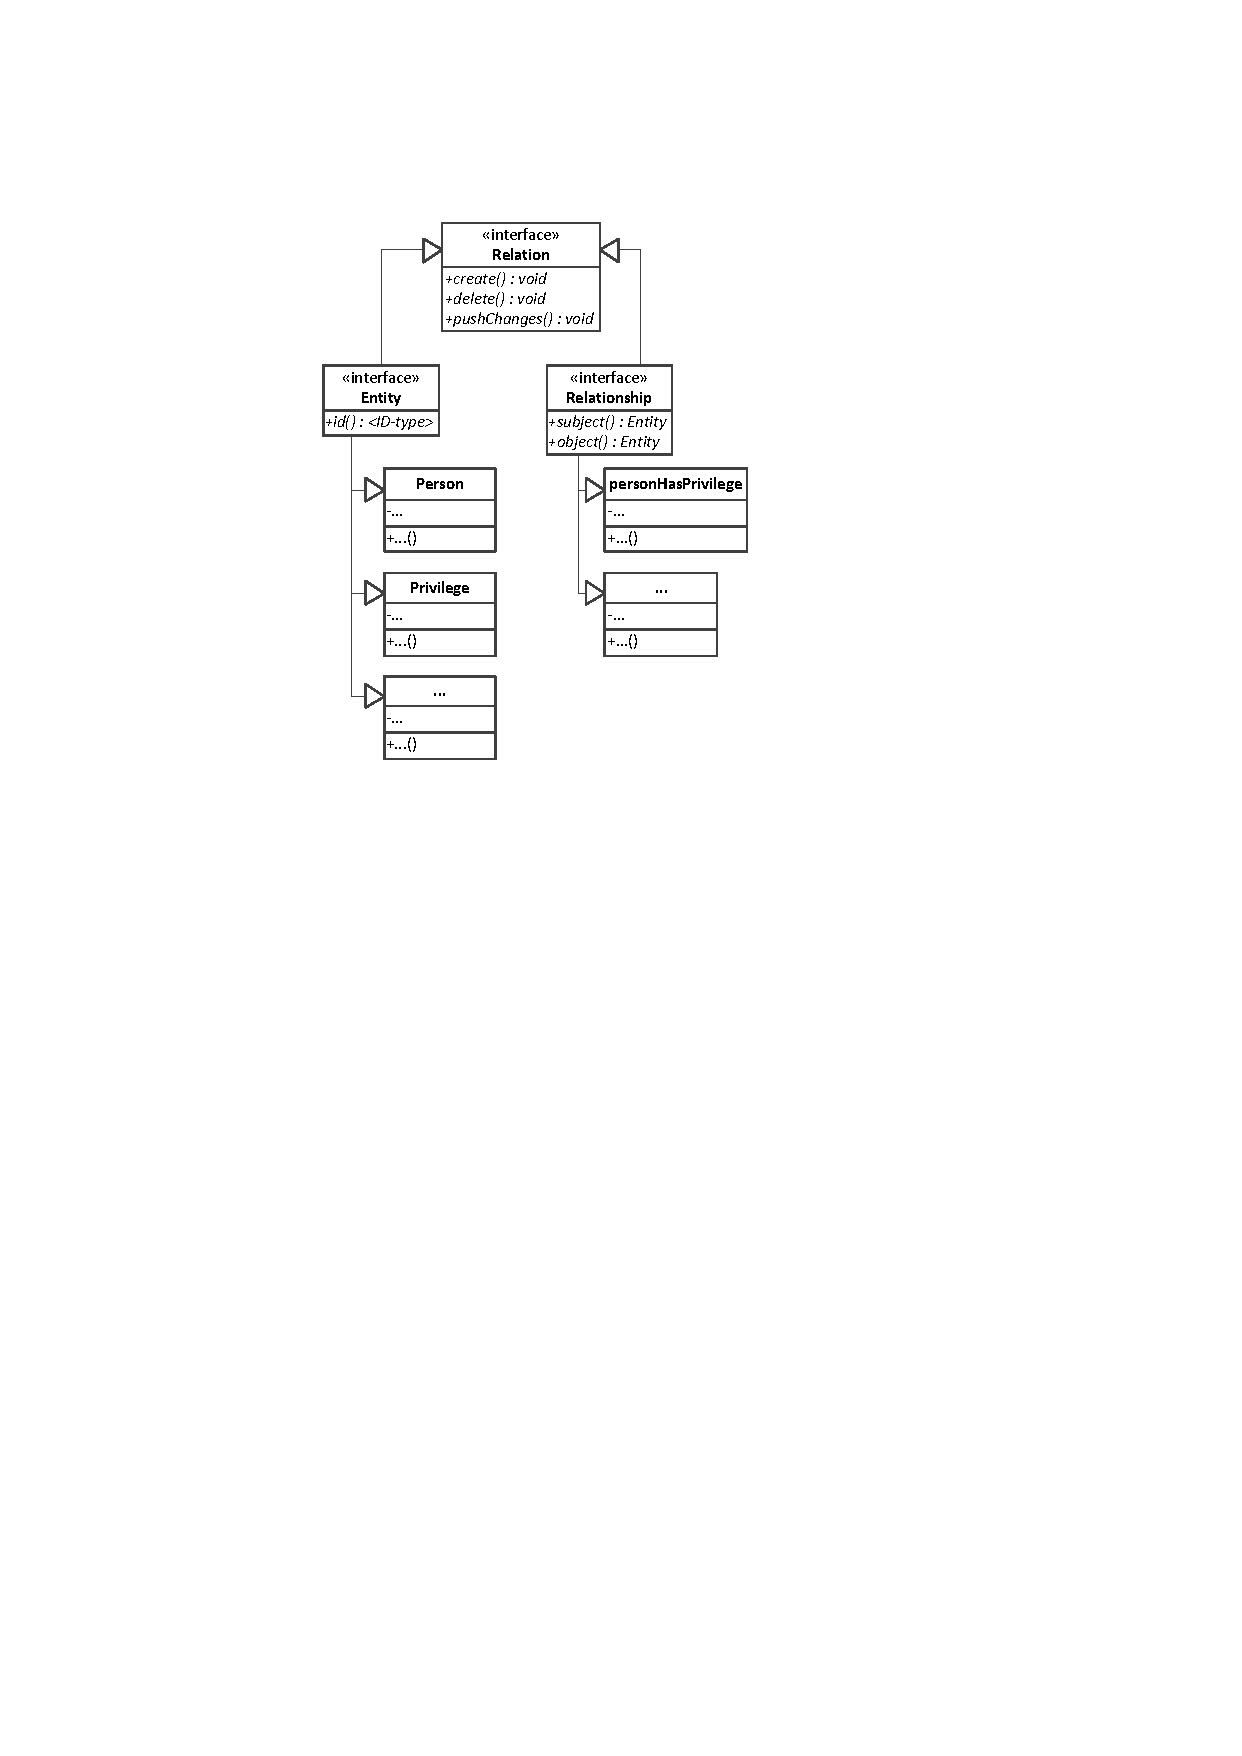
\includegraphics[width=\columnwidth]{images/UML-active-records.pdf}
	\caption{Overall structure of the active records}
	\label{fig:data-access-layer}
\end{figure}

\end{multicols}
\begin{multicols}{2}[\subsection{Web application}]

\begin{figure}[H]
	\centering
		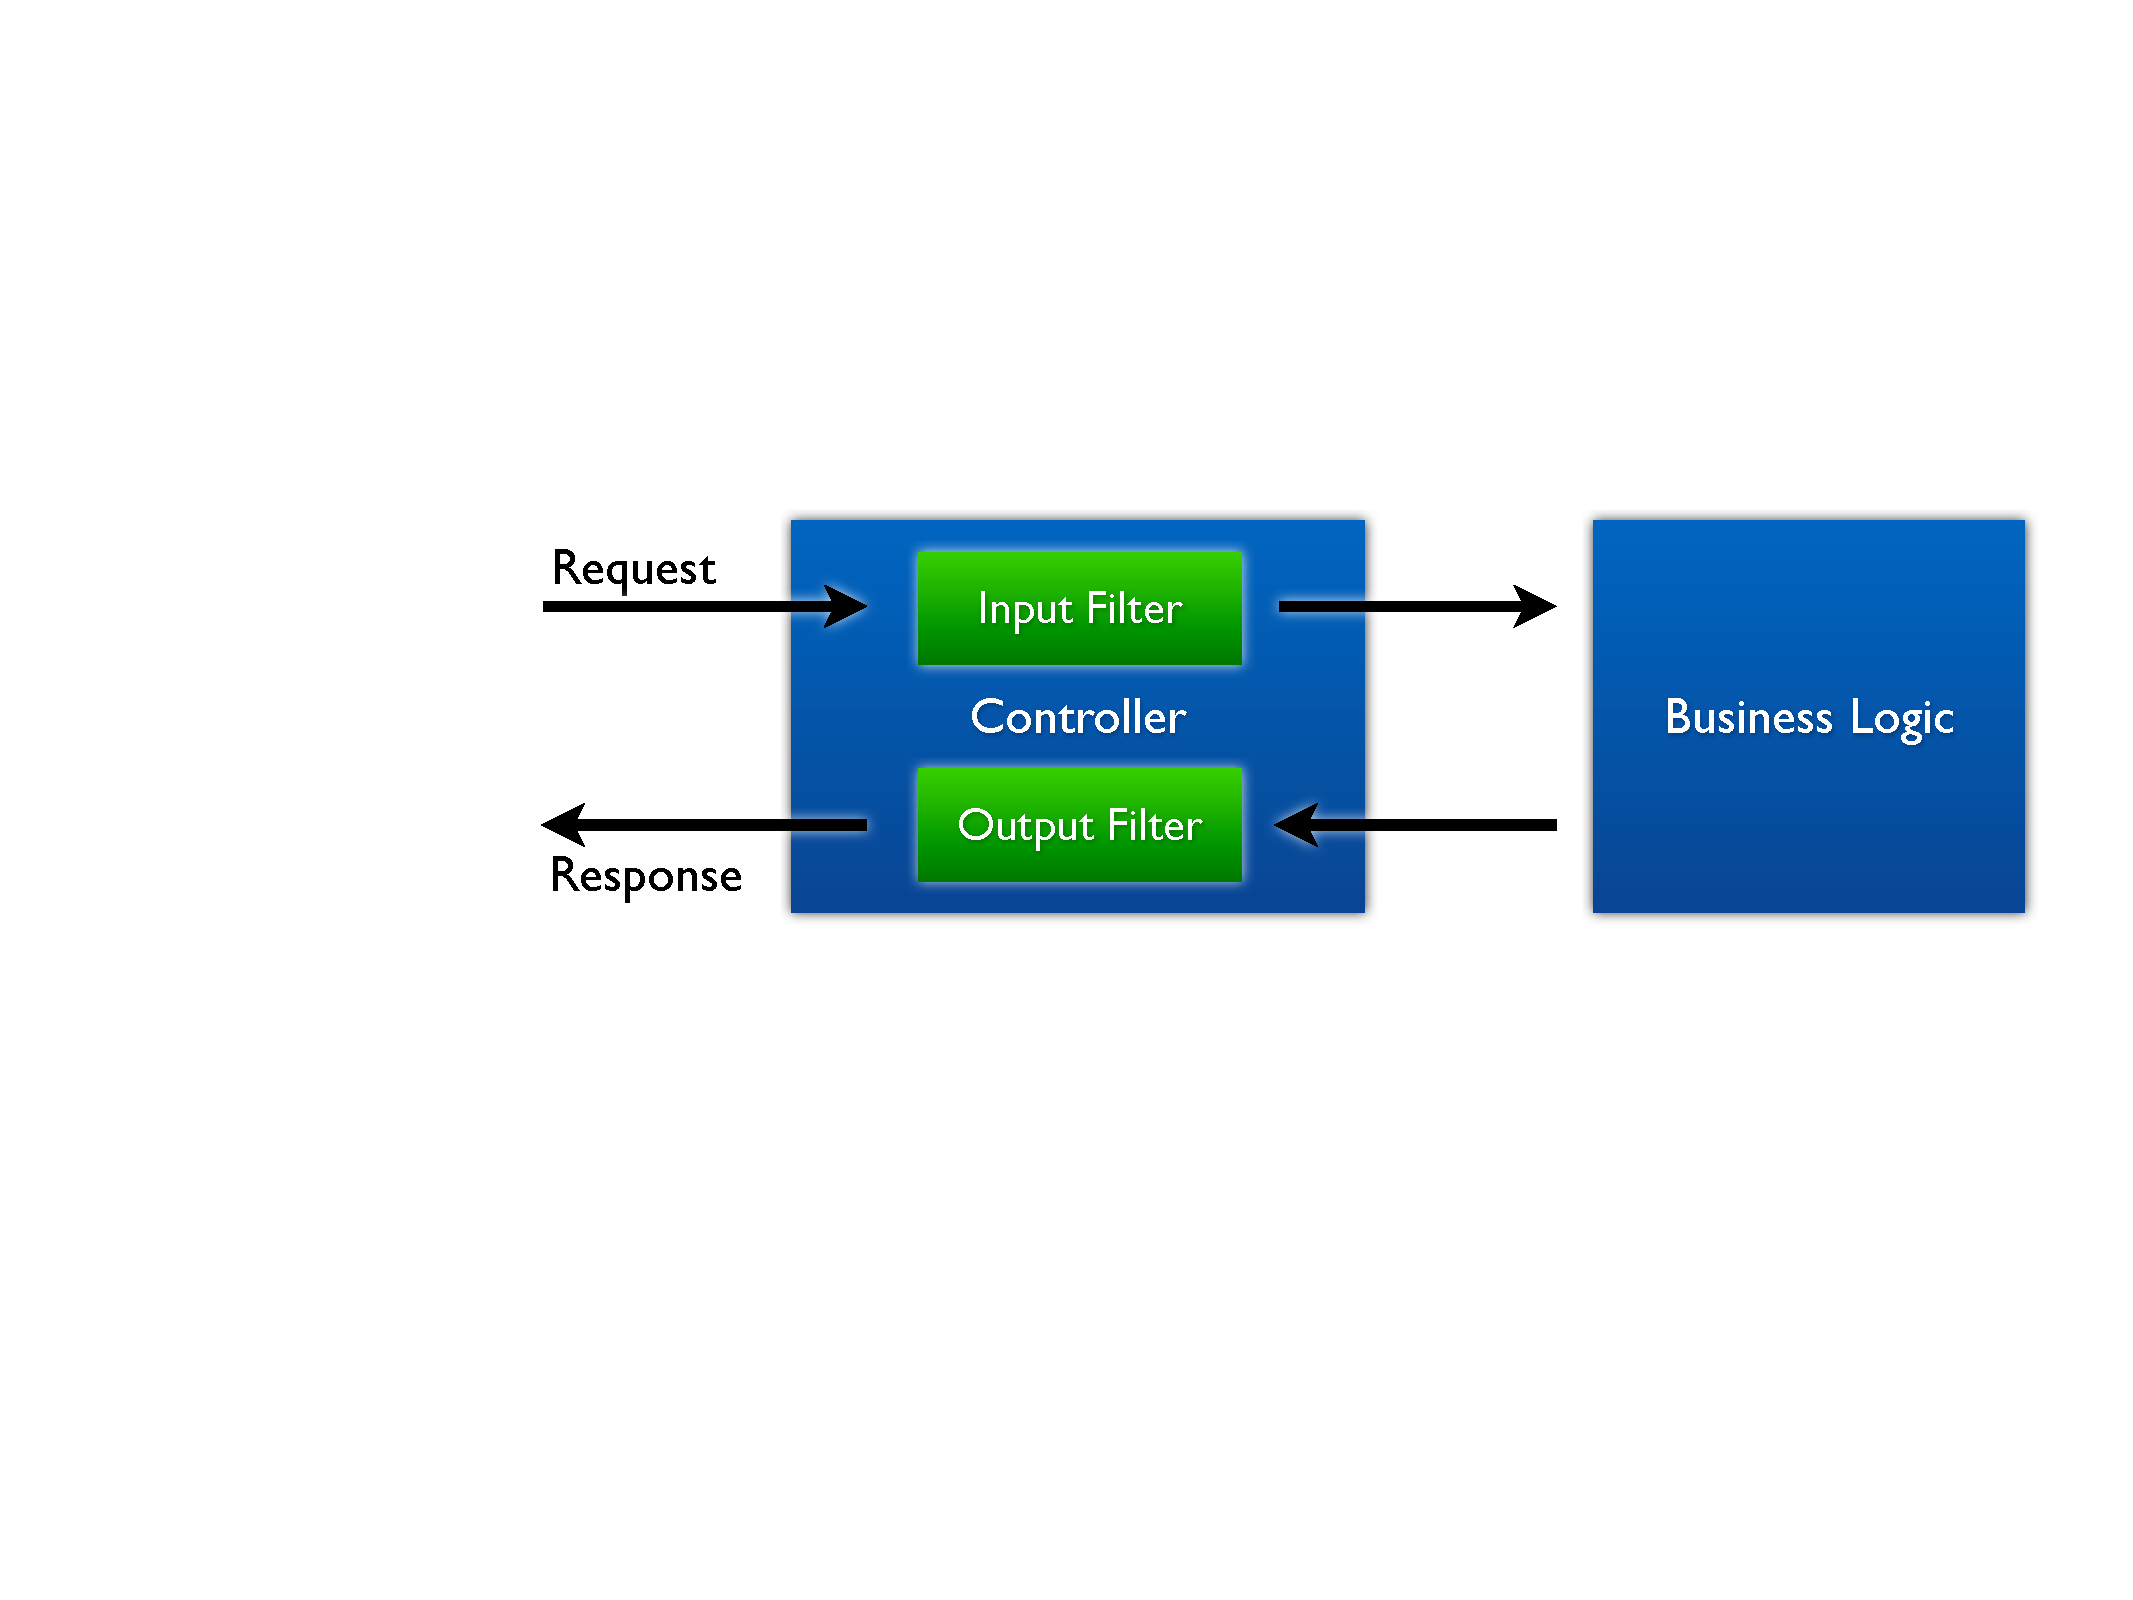
\includegraphics[width=\columnwidth]{images/design_webapplication.pdf}
	\caption{Data flow within our web application.}
	\label{fig:design-web-application}
\end{figure}

Our web application is, as stated in \autoref{sec:architecture}, layered into multiple loosely coupled tiers. Communication between these tiers takes place in strictly specified ways. A request to the system is issued by the user, which directly interacts with the front end through a web browser. It is than processed by a controller, which handles input sanitizing and validating. The controller invokes the business logic which returns structured data (XML in our case). Using XSL-T that data is transforrmed into whatever format is requested and sent back to the front end by the controller.

\begin{description}
\item[Controller] The core of our application is a Servlet according to the Java Servlet Specification. It provides the business layer with session handling and offers access to the data access layer (which is then invoked directly from within the business layer). The main purpose of the Controller is to route data from the front end to the business layer and vice versa. Since no direct access from the front end to the business layer is possible, user privileges are also checked within the controller, so that it is not even possible to pass data to a module of which a user lacks the privilege to make use of.

\item[Modules] To achieve the decoupling of business logic from the controlling unit, we encapsulated it into Modules. These Modules are to be loaded on server startup and provided with an environment; that is, a \emph{RelationManager} for accessing the database. Using Javas Annotation API, the Module classes are provided with information on how the controller should treat them. For example, a method may be annotated with \texttt{@Action}, which declares this method as accessible via the servlet. The Controllers task will then be, to map incoming request to that method. Modules are expected to return a \texttt{org.w3c.dom.Document}\link{http://download.oracle.com/javase/6/docs/api/org/w3c/dom/Document.html}{org.w3c.dom.Document}, which can than be processed by the controller.

\item[OutputConverter] OutputConverter are used for transforming the XML Document which is returned by the business layer into a certain format.

\item[InputConverter] In order to deal with user data, an special mechanism was designed. Data classes which represent forms are provided with declarative information via Annotations. These are to be processed by the Controller to transaprently make the data accessible to the business layer. These form classes are very similar in spirit to Active Records in the data access layer, since they are used to access data as well as transfer data.

\end{description}

\end{multicols}
\begin{multicols}{2}[\subsection{Scheduler algorithm}]

The problem of course scheduling is known to be NP-hard \cite{JSSP}. The course scheduling problem can be approached by using search algorithms. As a matter of fact this works for simple cases only. Course scheduling, especially at universites and similiarly large facilities, goes along with complex constraints. With increasing input and more constraints an optimal solution cannot be computed within a reasonable amount of time. The widely used approach of using a genetic algorithm seemed to be promising and was therefore chosen for our project.

Genetic algorithms are a subset of the metaheuristic optimization algorithms. Metaheuristics, being part of stochastic optimization, are algorithms using randomness to some degree in order to find solutions to hard problems where the solutions are optimal or as optimal as possible. Metaheuristics are applied when little is known about what the optimal solution looks like. Heuristics are hardly useful as neccessary information is lacking. Brute-force is out of question as the space of possible solution is too large. However, when a candidate solution is given it can be rated in order to evaluate how good it is indeed \cite{Luke2009Metaheuristics}.

In order to understand the scheduler algorithm the genetic algorithm operations, \emph{setup}, \emph{fitness function}, \emph{crossover}, \emph{mutate} and \emph{selection}, are best conceived of as core components of the scheduler algorithm. These operations are described below.

\begin{description}
\item[Setup] generates the initial population of candidate solutions in a random or semi-random way. A candidate solution is created when every course is allocated in a room at a given time. The \emph{setup} process is finished when $\lambda$ candidate solutions were created.

\item[Fitness function] rates the candidate solution assigning it a score. The score is mapped to the number of constraints satisfied. The more constraints are satisfied the higher the candidate solution is scored. The score ranges from $0.0$ to $1.0$.

\item[Crossover] creates a new candidate solution by mixing and matching parts of two given candidate solutions. How the mixing and matching is done depends to the representation of a candidate solution. As our representation is a mapping of courses to allocated rooms and times, these allocations are mixed and matched.

\item[Mutation] creates a new candidate solution by taking a given candidate solution and changing a specified amount of course allocations to new, randomly chosen, course allocations.

\item[Selection] iterates the given candidate solutions and keeps only the $\mu$ best solutions. The solutions are selected, according to the score given by the \emph{fitness function}, through dropping the rest of the candidate solutions.
\end{description}

It is also possible that the desired scheduling is not scheduleable at all, for instance when two courses have the hard constraint to be placed at the same room with overlapping time. In this case the scheduling is stopped and the user has to resolve the constraint conflict on their own.

% Figure \ref{fig:schedulercomponents} illustrates the components interaction.

\begin{figure}[H]
	\centering
		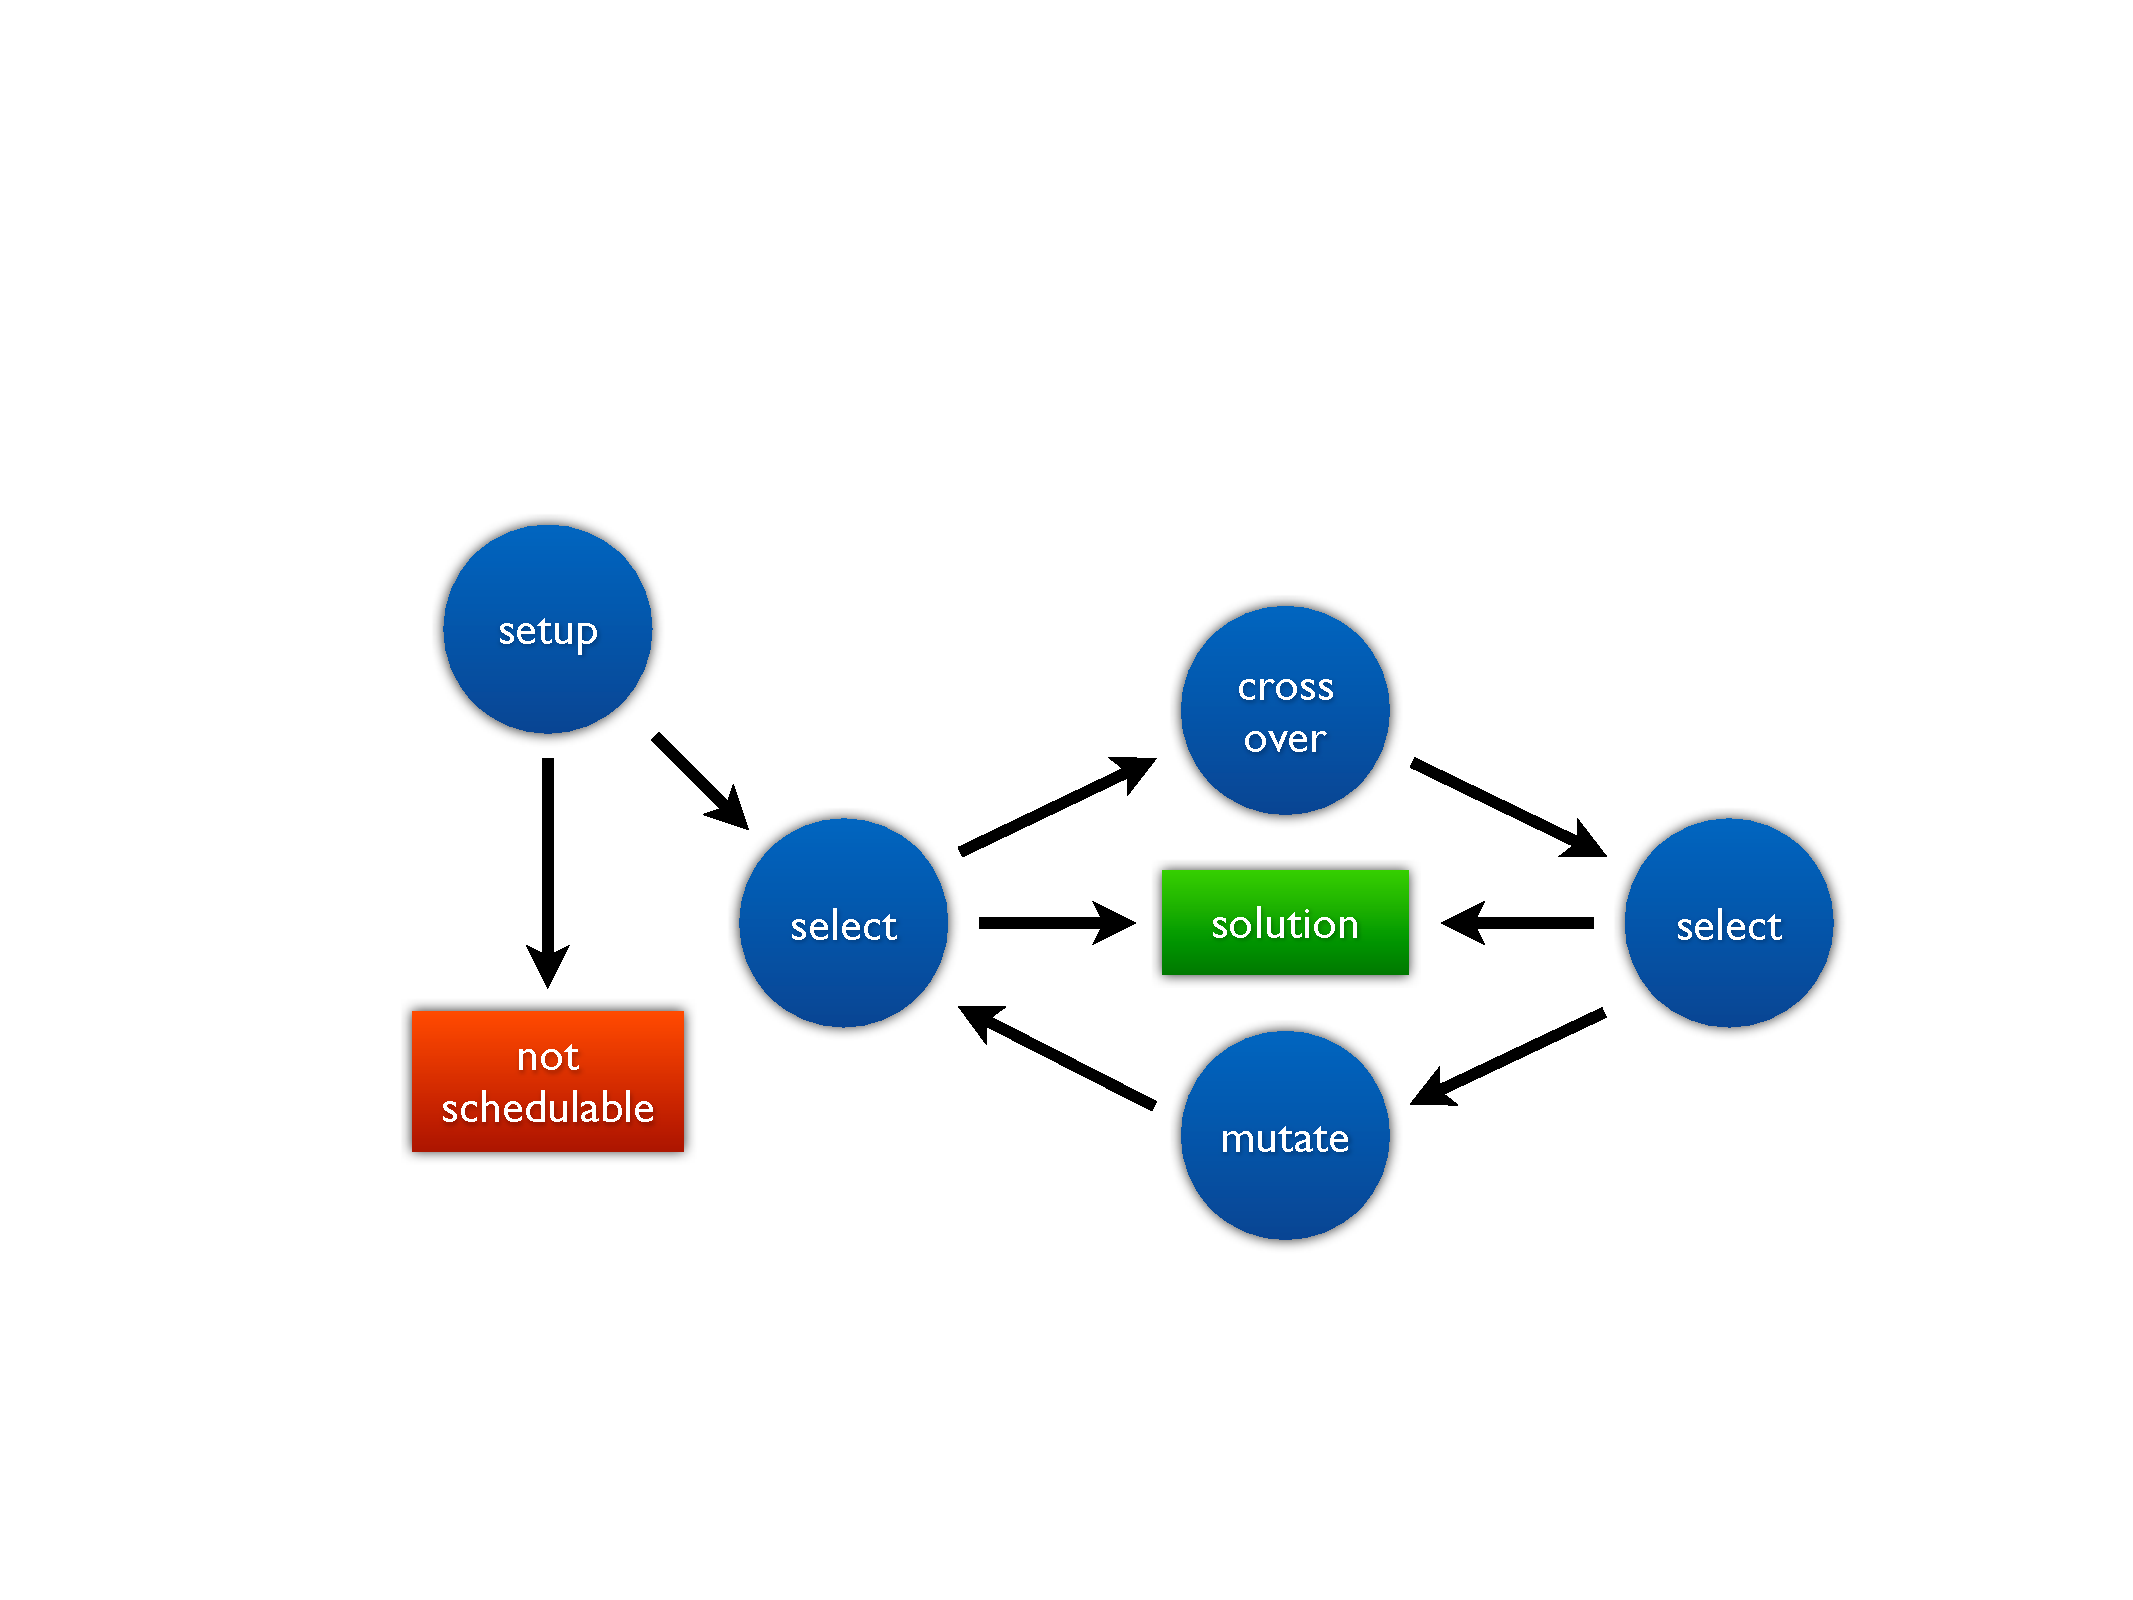
\includegraphics[width=\columnwidth]{images/algorithm.pdf}
	\caption{Routine of the scheduler algorithm. An initial population of candidate solutions is generated. Every candidate solution is rated. If non-solvable conflicts appear the scheduling has to be terminated. Otherwise the setup phase is followed by optimizing the candidate solutions through applying crossover and mutation operations until an optimum schedule is found.}
	\label{fig:schedulercomponents}
\end{figure}
